\begin{abstract}
RL with verifiable rewards often treats task curricula and failure
recycling as estimator-agnostic. We ask what task-level activity the
deployed group estimator makes available to either intervention. For the
practical MaxRL convention that drops all-fail groups, the expected
absolute coefficient mass over $N$ i.i.d.\ binary rollouts is exactly
$2(\passat{N}-\passat{1})$ --- the estimator's own pass@$N$ gap. The
score's peak moves toward harder tasks as $N$ grows, it recovers the
common learnability score $p(1-p)$ at $N=2$, and dropping all-fail groups
shifts the truncation order to $N-1$. It is an estimator-side diagnostic,
not a theorem of learning progress. Rollout-aware selection carries
empirical content: in a fresh 20-seed Acrobot tournament at $N=16$,
sampling by the deployed-$N$ score improves target-uniform AUC over
$p(1-p)$ by $+.0480$ (95\% paired-bootstrap CI $[+.0209,+.0738]$) and
over uniform sampling as well. Its scope is bounded by design: in an
exact-probability Digits counter-test the mismatched RLOO estimator
prefers the same sampler, rejecting a universal estimator-to-sampler
mapping, and an externally recorded six-block maze factorial reports
higher time-integrated coverage under MaxRL than under GRPO in 6/6 blocks
under each sampler at common optimizer settings --- an
estimator-conditioned ordering, not universal superiority. A reported
three-seed Countdown aggregate couples higher mean@16 with a lower logged
VERL bootstrap best@16 coverage proxy under a deployed recycling package,
motivating $\passat{k}$ recomputed from retained raw outcomes.
Data-selection interventions should be evaluated with the estimator
beneath them, and coefficient activity treated as a source of curriculum
hypotheses, not a universal curriculum objective.
\end{abstract}

\section{Introduction}

RL with verifiable rewards (RLVR) converts automatically checkable outcomes
into policy updates, but every update first pays for a group of model
rollouts. Two data-level interventions
try to make that budget productive. A \emph{difficulty curriculum} samples
tasks believed to be learnable now; \emph{failure recycling} relabels a failed
trajectory as a verified success for a task it actually achieved. Both are
often evaluated as portable modules, separately from the estimator that turns
their sampled data into gradients.

That separation is fragile. Group-relative estimators emit no contrast when
all $N$ samples agree, while success-conditioned estimators may drop all-fail
groups entirely. Variance normalization can continue weighting near-mastered
prompts after a success-conditioned estimator has released them. Relabeling
changes the achieved-task distribution toward outputs the current policy
already reaches. A sampler, recycler, and estimator can therefore move
training mass toward different parts of the task pool even when all are
described as improving efficiency.

We organize these interactions around the expected absolute coefficient mass
emitted by the deployed estimator before accounting for score-gradient
direction or magnitude. For practical MaxRL \citep{maxrl}, this mass is
\[
A_N(p)=2\{1-(1-p)^N-p\}=2(\passat{N}-\passat{1}).
\]
Its two zeros separate a dead zone, a learnable region, and a mastered tail.
Its peak moves toward harder prompts as the rollout count grows. Coefficient
mass is not a proof of learning progress, but it is estimator-side activity a
task sampler can predict before purchasing a group of rollouts.

This view yields three contributions:
\begin{enumerate}
\item \textbf{Exact rollout-aware coefficient activity.}
We derive $A_N$, its peak and asymptotics, and show that the practical
drop-all-fail estimator targets truncation order $T=N-1$, not $N$; a
fixed-completion sweep checks its nontrivial $N$ dependence. The identity
is an estimator-side diagnostic, not a learning theorem.
\item \textbf{A positive--negative pair that maps the score's scope.}
In fixed-pool Acrobot, $u_{16}$ is supported over both $p(1-p)=u_2$ and
uniform sampling by the frozen rule.
In a separate paid-probe Acrobot family, registered $u_{16}$ superiority over
ProCuRL selection is unsupported and probe cost dominates all three probed arms.
In an exact-probability Digits counter-test, the internally frozen
interaction fails, mismatched RLOO prefers the same sampler, and neither
matched sampler beats uniform --- so the supported content is rollout-aware
difficulty targeting, not estimator matching. The pair is itself the
contribution: it locates the
boundary inside which the activity score is informative, rather than
reporting a uniformly positive story.
\item \textbf{Coverage accounting on neural gradients.}
At common optimizer settings, the externally recorded fresh maze wave has
higher MaxRL than GRPO coverage in all six blocks under each sampler. A
reported three-seed Countdown aggregate shows higher average correctness but
lower VERL bootstrap best@16 under a deployed recycling package. We preserve
the registration, artifact, metric, and dose limitations of both results.
Both motivate an operational recommendation: report mean@$k$ beside
$\passat{k}$ computed from retained task outcomes whenever a data-selection
intervention ships.
\end{enumerate}

The paper is deliberately narrower than the full project record:
exploratory mechanisms, failed hypotheses, robotics pilots, gate studies,
and implementation detail remain in the appendix and artifact.

\section{Coefficient activity under practical MaxRL}
\label{sec:theory}

\paragraph{Setup.}
For task $x$, let $r_i\in\{0,1\}$ be $N$ conditionally independent rollout
rewards with pass rate $p=p_\theta(x)$ and $K=\sum_i r_i$. Let
$s_i=\nabla_\theta\log\pi_\theta(y_i\mid x)$ be the response score and
$\hat g=\sum_iw_i s_i$ the group update. Then
$\passat{N}=1-(1-p)^N$. We analyze the zero-stabilizer idealization of the
released practical centered MaxRL convention, which assigns
\[
w_i=\frac{r_i}{K}-\frac1N\quad\text{when }K>0,
\qquad w_i=0\quad\text{when }K=0.
\]
All-pass groups also have zero contrast. The released implementation uses a
finite denominator stabilizer $\varepsilon$; for $K>0$ this multiplies the
ideal coefficients by $K/(K+N\varepsilon)$. Thus the identities below are
exact for the stated zero-$\varepsilon$ convention rather than for its
finite-$\varepsilon$ magnitude.

\begin{lemma}[Practical truncation order]
\label{lem:trunc}
The expectation of the drop-$K=0$ practical estimator equals the gradient of
the $(N-1)$-term truncated maximum-likelihood objective, not the $N$-term
objective.
\end{lemma}
\noindent
For $J_T(p)=-\sum_{t=1}^{T}(1-p)^t/t$, direct conditioning gives
\[
\mathbb E\hat g
=\left(\frac{1-(1-p)^N}{p}-(1-p)^{N-1}\right)\nabla p
=\left(\sum_{j=0}^{N-2}(1-p)^j\right)\nabla p
=\nabla J_{N-1}.
\]
The correction matters whenever a theoretical truncation parameter is mapped
to a deployed group size. Details and the non-dropped control-variate
convention are in App.~\ref{app:proofs}.

\begin{proposition}[Exact coefficient mass]
\label{prop:mass}
The expected absolute coefficient mass of the practical estimator is
\[
A_N(p)=\mathbb E\!\left[\sum_{i=1}^{N}|w_i|\right]
=2\{1-p-(1-p)^N\}
=2(\passat{N}-\passat{1}).
\]
\end{proposition}
\noindent
For a mixed group with $0<K<N$, successes and failures each contribute
$(N-K)/N$ absolute mass. Therefore
\[
A_N(p)=\frac{2}{N}\mathbb E[(N-K)\mathbf1\{K>0\}]
=2\{(1-p)-(1-p)^N\}.
\]
This identity concerns coefficients, not gradient norm, signal-to-noise
ratio, or expected improvement: score-gradient geometry can change its
downstream effect.

The bridge to the expected update is nevertheless exact. With
$\mu_+=\mathbb E[s_i\mid r_i=1,x]$ and
$\mu_-=\mathbb E[s_i\mid r_i=0,x]$,
\[
\mathbb E[\hat g\mid x]=u_N(p)(\mu_+-\mu_-),
\qquad u_N(p)=A_N(p)/2.
\]
Thus $u_N$ is the estimator-controlled scalar factor in the expected update;
the conditional score geometry remains outside the mass calculation.

\begin{figure}[t]
\centering
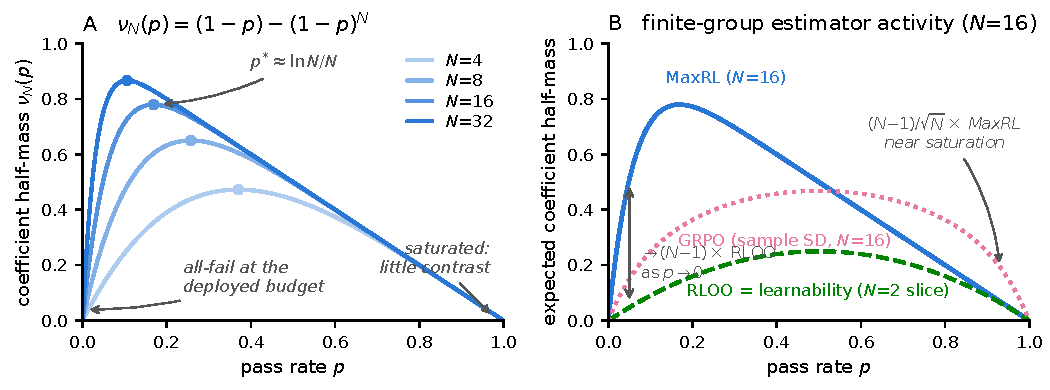
\includegraphics[width=.84\linewidth]{figures/fig1_utility}
\caption{\textbf{Estimator-conditioned activity.}
\emph{Left:} $u_N=A_N/2=\passat{N}-\passat{1}$ for several rollout
counts; its peak is derived rather than tuned and moves toward harder tasks
as $N$ grows. \emph{Right:} exact expected half-mass at $N=16$ under
zero-stabilizer MaxRL, standard gradient-averaged RLOO, and the
zero-stabilizer sample-SD-normalized GRPO convention. Coefficient
mass is sign-blind, so the curves motivate rather than prove the empirical
coverage ordering.}
\label{fig:utility}
\end{figure}

\paragraph{Consequences.}
The derivative of $u_N(p)=1-p-(1-p)^N$ gives the unique peak
\[
p_N^\star=1-N^{-1/(N-1)}\simeq\frac{\log N}{N}.
\]
Thus the relevant intermediate difficulty depends on rollout budget. At
$N=2$, $u_2=p(1-p)$, coinciding with a common learnability score. As
$p\to0$, MaxRL carries $(N-1)$ times the coefficient mass of standard
$1/N$-averaged RLOO. As $p\to1$, MaxRL and RLOO both decay at first order in
$1-p$, whereas
sample-SD-normalized GRPO allocates relatively more mass to near-mastered
prompts (App.~\ref{app:proofs}).

\paragraph{Fixed-completion check.}
We tested the arbitrary-$N$ prediction on a 36-task CPU skill-chain testbed
with $N\in\{2,4,8,16,32\}$, eight paired seeds, no recycling, and exactly
51,200 sampled completions per cell. Teacher decay was normalized per
completion so changing $N$ did not silently change its memory horizon.

\begin{table}[t]
\centering
\small
\setlength{\tabcolsep}{5pt}
\caption{\textbf{Post-guidance CPU check.} Mean normalized pass-rate AUC
differences at fixed sampled-completion budget. Seed signs are descriptive;
the sweep was not pre-registered.}
\label{tab:nsweep}
\begin{tabular}{@{}lrrrrr@{}}
\toprule
$N$ & 2 & 4 & 8 & 16 & 32\\
\midrule
$u_N-p(1-p)$ & .0000 & +.0307 & +.0920 & +.1526 & +.1909\\
$u_N-\mathrm{uniform}$ & -.0106 & -.0032 & +.0309 & +.0453 & +.0836\\
wins vs.\ $p(1-p)$ & identical & 8/8 & 8/8 & 8/8 & 8/8\\
\bottomrule
\end{tabular}
\end{table}

The $N=2$ identity reproduces bit-for-bit. For every $N>2$, the
rollout-aware utility beats the score-only $p(1-p)$ comparator in all paired
seeds. The mean gap increases across tested $N$, but only 5/8 seed
trajectories are monotone, so we do not claim a scaling law. Nor does $u_N$
universally beat uniform: the mean contrast becomes positive only at $N\ge8$.
The paired positive-seed counts are 3/8, 3/8, 8/8, 7/8, and 7/8 as $N$
increases. This is evidence
for rollout awareness in one co-designed testbed, not a blanket curriculum
advantage or an algorithm-level comparison with prior work.

\paragraph{Exact-probability counter-test.}
The stronger test does not generalize the sampler mapping. Under an internally
hashed local protocol without an immutable public pre-execution commit, a fresh
24-block Digits contextual bandit computes the policy's correct-class probability
exactly before every update. Its internally frozen
estimator-by-sampler interaction is $+.01589$ (95\% CI
$[-.01686,+.04712]$, exact sign-flip $p=.350$; 15/24 positive) and is not
supported. MaxRL favors $u_8$ over $p(1-p)$ by $+.20842$, but RLOO also favors
$u_8$, reversing its prediction; both estimator-matched samplers are below
uniform. The activity algebra therefore generates testable hypotheses, not a
universal learnability or curriculum-optimality law.

\section{From mass to interventions}
\label{sec:method}

\paragraph{Task sampling.}
FrontierMax operationalizes the identity without changing the within-group
estimator. Each task maintains discounted Beta evidence, draws a posterior
pass rate $\tilde p_x$, and samples approximately as
\[
q(x)=\frac{\epsilon}{M}
 +(1-\epsilon)\frac{[u_N(\tilde p_x)]^\gamma}
 {\sum_{j=1}^{M}[u_N(\tilde p_j)]^\gamma}.
\]
The floor $\epsilon$, concentration $\gamma$, decay, and posterior
estimator remain empirical choices; the theory contribution is the utility
and its $N$-dependence, not a parameter-free scheduler.

\paragraph{Failure recycling.}
For an all-fail request, a verified achieved goal can create an auxiliary
update where repeating that request would emit none. This requires an exact
verifier and rewriting any goal-bearing conditioning. Even then, the achieved
goal is selected from a failed group and generally does not yield an unbiased
fresh-task policy gradient. We treat recycling as a verified auxiliary
update. It changes both update dose and direction, while the achieved-goal
distribution is biased toward what the policy already reaches
\citep{her,gcsl}.

\paragraph{Predictions.}
The mass curves motivate, but do not prove, two empirical expectations.
First, MaxRL and variance-normalized GRPO can exhibit different coverage
orderings under a common sampler; this need not imply a sampler-by-estimator
interaction. Second, the deployed recycling package may trade a coverage proxy for
mean accuracy when it concentrates updates on reachable outputs. Both require
controlled measurement.

\section{Evidence}
\label{sec:evidence}

The four families support distinct claims. The maze factorial tests the
estimator-conditioned coverage ordering on real neural gradients; the
Acrobot tournament isolates the deployed-$N$ score shape under a fixed
scaffold; the paid-probe comparison prices probe-based selection under a
shared budget; and the Countdown record supplies the applied
mean-versus-coverage observation that motivates raw-outcome reporting. The
score's positive support is deliberately small-scale and fully controlled;
the neural families test estimator-side predictions, not the score.

\subsection{Externally recorded fresh-wave maze result}

\paragraph{Design.}
The testbed is a 1.26M-parameter transformer trained on procedurally generated
$17\times17$ mazes. Each balanced block shares a seed, warm start, task pool,
and evaluation schedule across
$\{\text{MaxRL},\text{GRPO}\}\times
\{\text{uniform},\text{FrontierMax}\}$. The outcome is time-integrated
$\passat{8}$ coverage relative to the warm-start checkpoint, not final
reward, at identical deployed optimizer settings with no per-estimator
learning-rate tuning.

Each run uses $N=32$, eight prompt groups per training step, and 250 steps.
Evaluation occurs every 25 steps on 16 held-out mazes per level; coverage
AUC is the mean $\passat{8}$ over steps 25--250 minus the warm-start value.

The first factorial rejected its stronger externally recorded endpoint claim
(3/6 uniform and 4/6 FrontierMax blocks with the predicted sign), and we
retracted the earlier zero-exception cohort claim. Wave-1 time-integrated
coverage was positive in all blocks under each sampler, but that outcome was
discovered exploratorily; the external record specifies it as wave 2's
primary, with a falsification rule, before new seeds ran, though the locking
commit object is not vendored in this checkout.

\begin{figure}[ht]
\centering
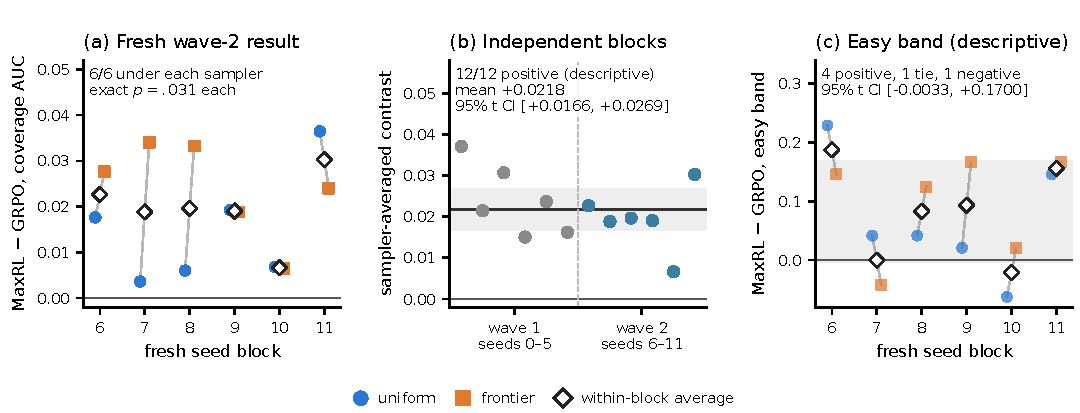
\includegraphics[width=.94\linewidth]{figures/fig_maze_block_contrasts}
\caption{\textbf{Maze factorial at the independent seed-block unit.}
\emph{(a)} The externally recorded fresh-wave result is positive in 6/6 blocks under each
sampler (exact sign $p=.03125$ each). Connected observations share a block.
\emph{(b)} Sampler-averaging gives wave-2 mean $+.0195$ and post-hoc 95\% CI
$[+.0115,+.0275]$; 12/12 cross-wave block averages are descriptive.
\emph{(c)} Easy-band localization is suggestive: four positive blocks, one
tie, one negative, and an interval containing zero.}
\label{fig:maze}
\end{figure}

\paragraph{Result.}
The wave-2 primary is positive in all six fresh blocks under uniform
sampling and all six under FrontierMax (exact two-sided sign $p=.03125$ per
sampler). Six blocks put this sign test at its granularity floor (6/6 is
the only outcome clearing $.05$; the frozen 5/6 bar could not), so the
inferential anchor is the block-averaged mean: averaging the correlated
sampler observations within each block yields $+.0195$, post-hoc 95\% $t$
interval $[+.0115,+.0275]$, with every leave-one-block-out interval above zero.
Across both waves, all 12 block averages are positive, but that statement is
descriptive because wave 1 selected the outcome.

The data support an estimator-conditioned coverage ordering at common
deployed optimizer settings, not universal estimator superiority or the
strong mechanism account we initially expected. The recorded pair-level
easy-band criterion was met, yet block aggregation leaves four positive, one
tied, and one negative easy-band contrast with an interval crossing zero.
Localization therefore remains suggestive. We froze an AUC robustness
multiverse, but the checkpoint trajectories required to evaluate its warmup,
integration, and horizon variants remain external
(App.~\ref{app:protocols}).

\subsection{Fresh fixed-pool Acrobot score test}

We next isolate the arbitrary-$N$ score on official Gymnasium
\texttt{Acrobot-v1}. Eight nested tip-height predicates share one task-blind
H64 actor (640 parameters); the hardest predicate is exactly native Acrobot
success. All arms use practical MaxRL with $N=16$, no hindsight, learning
rate $3\times10^{-4}$, and a nominal two million paid environment
transitions. Twenty fresh paired seeds compare uniform sampling, the
common-scaffold $p(1-p)=u_2$ score, and $u_{16}$ under identical discounted
Beta tracking. The internally frozen primary is target-uniform normalized
transition-AUC --- evaluation success averaged uniformly over the eight
predicates, integrated over the paid-transition axis, and normalized by the
budget --- for $u_{16}-p(1-p)$, with support requiring a positive exact
two-sided sign-flip test at $.05$ and a point estimate of at least $+.01$.

\begin{table}[ht]
\centering
\scriptsize
\setlength{\tabcolsep}{3.2pt}
\caption{\textbf{Fresh Acrobot tournament.} Paired differences use 20 fresh
seeds under the source/runtime-locked protocol. The two uniform comparisons
form one Holm family.}
\label{tab:acrobot}
\begin{tabular}{@{}lrrrrl@{}}
\toprule
contrast & mean $\Delta$ & 95\% boot.\ CI & exact $p$ & Holm $p$ & decision\\
\midrule
$u_{16}-p(1-p)$ & +.0480 & [+.0209,+.0738] & .0034 & -- & supported by rule\\
$p(1-p)-$uniform & -.0062 & [-.0226,+.0122] & .5078 & .5078 & not supported\\
$u_{16}-$uniform & +.0419 & [+.0218,+.0606] & .0008 & .0016 & supported\\
\bottomrule
\end{tabular}
\end{table}

The arm means are $.64523$ (uniform), $.63907$ ($p(1-p)$), and $.68711$
($u_{16}$). The primary clears both frozen criteria; 15/20 paired differences
are positive. The result therefore supports the deployed-$N$ score shape
against its $N=2$ ablation in this fixed family, while the $p(1-p)$ arm itself
is not supported over uniform by the frozen secondary test.

The mean $u_{16}-p(1-p)$ contrasts remain descriptively positive on
sampled-group ($+.05294$) and optimizer-update ($+.05366$) axes. $u_{16}$
also receives 2.40 fewer groups and 3.42 fewer updates per million
transitions, so it did not win by receiving more updates; these
non-confirmatory axes do not identify a causal mechanism. Native-success
transition-AUC is $.31085$, $.30521$, and $.37615$ across the three arms.
App.~\ref{app:protocols} reports the near-equal observed mass means between
adaptive arms and records the audited but RNG-confounded precursor
separately.

\subsection{Paid-probe ProCuRL confirmatory comparison}

A separate frozen family tests source-faithful ProCuRL environment-selection
semantics, not merely the $p(1-p)$ score on a shared posterior. On the same
eight-task Acrobot family and 640-parameter practical-MaxRL learner, 80 paired
seeds compare ProCuRL selection, range-matched $u_{16}$, a paid-probe uniform
sham, and ordinary uniform. The three probed arms refresh 20-episode-per-task
estimates every 5,120 student transitions and charge every probe transition to
the common two-million paid budget. The internally frozen fixed-paid-AUC contrast
$u_{16}-$ProCuRL is $+.00489$ (paired $t_{79}=1.977$, $p=.0515$;
percentile-bootstrap 95\% CI $[+.00011,+.00973]$). The bootstrap interval
excludes zero while the frozen $t$ criterion fails, but the verdict does
not hinge on that: the point estimate misses the frozen $.02$ SESOI
fourfold, so the rule is unsupported either way.
Neither adaptive-versus-sham secondary
rejects after Holm correction (adjusted $p=.4568$ and $.4547$); this
non-rejection is not an equivalence claim. Probes consume about 93.2\% of paid transitions; the
three probed arms trail ordinary uniform by $-.314$, $-.309$, and $-.312$
AUC, respectively (all Holm-rejected). Thus this cadence diagnoses probe-cost
domination, not general ProCuRL inferiority or a reproduction of its complete
PPO system; in RLVR loops whose pass-rate posteriors update free of charge
from training rollouts, probe accounting is a property of probing semantics
rather than of posterior-based selection. This 80-pair family and multiplicity plan are separate from
Table~\ref{tab:acrobot}; full accounting is in App.~\ref{app:protocols}.

\subsection{Countdown recycling: accuracy up, coverage proxy down}

\paragraph{Design.}
We fine-tune SmolLM2-360M on exact-verifier Countdown tasks with $N=16$.
The retained comparison is a three-seed aggregate on a fixed 128-task tier-1
evaluation set at step 60. Mean@16 measures average correctness over samples;
the logged VERL best@16 metric applies 1,000 with-replacement resamples of
size 16 to each prompt's 16 binary outcomes and averages whether a resample
contains a success. Conditional on $c$ observed successes, it approximates
$1-(1-c/16)^{16}$. It is a bootstrap coverage proxy, not standard unbiased
$\passat{16}$ or the indicator that the observed set contains a success
\citep{codexpassk}. A summary-backed identity audit reports disjoint RL
train/evaluation pools, zero SFT overlap for tier 1, and 27/128 exposed tier-0
tasks. Tier 0 is excluded from absolute claims. The source manifests needed to
recompute those statements are not in this checkout. We retain this
historical aggregate because it motivated a frozen prospective replacement
protocol that recomputes standard observed-set $\passat{16}$ from retained
binary outcomes; until that protocol completes, we report the logged proxy
under its actual provenance rather than relabeling it.

\begin{figure}[H]
\centering
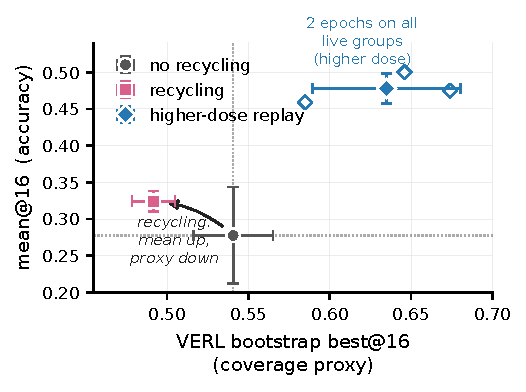
\includegraphics[width=.52\linewidth]{figures/fig_countdown_core}
\caption{\textbf{Countdown accuracy--bootstrap-coverage-proxy tradeoff.}
Error bars are sample standard deviations across three seeds; complete
three-seed B1/B2 records are not vendored (seed 3 is aggregate-only). The
reported recycling-package aggregate lies at higher mean@16 but lower VERL
bootstrap best@16. The live-group replay seeds use
two optimizer epochs on every live group, a substantially larger dose. This
higher-dose alternative improves both metrics but cannot separate dose from
update direction.}
\label{fig:countdown}
\end{figure}

\paragraph{Result.}
The reported recycling-package aggregate moves tier-1 mean@16 from
$.278\pm.066$ to $.324\pm.014$ while bootstrap best@16 moves from
$.541\pm.024$ to $.492\pm.013$ (mean $\pm$
sample SD across three seeds). The checkout lacks the complete three-seed
B1/B2 records, so we do not claim a paired seed test or per-seed sign
result, and we attach no name or effect claim to the aggregate. What it
demonstrates is the ambiguity itself: mean accuracy alone cannot reveal
whether coverage was spent to buy it, which is exactly why raw-outcome
$\passat{k}$ reporting matters.

An externally specified control applies two optimizer epochs to every live group
with hindsight disabled. It reaches mean@16 $.478\pm.021$ and
bootstrap best@16 $.635\pm.046$, with all three replay endpoints vendored.
Recycling permits at most 12 auxiliary groups per 64 requested groups
(18.75\%; realized dose can be lower), whereas replay doubles optimizer
epochs on every live group. It provides a higher-dose alternative that
improves both metrics, without decomposing relabel direction from update dose
or justifying a dose-monotonic causal bound.

Two negative results constrain the story. A favorable earlier gate setting
used faulty decay code; a corrected, externally specified strong-gate sweep behaved
like recycling-off and refuted the claimed monotone gate dial. A separate
Jugs suite collapsed under every arm because its learnable region was
effectively one template stratum. Neither the gate nor cross-domain
generality is a contribution here.

\section{Related work}

Our score is a distinct, testable functional form in a crowded
neighborhood: \emph{derived from the deployed estimator's own algebra},
with a peak that \emph{migrates with the rollout budget}, and used for
\emph{task selection rather than objective redesign}. Superiority over the
methods below is untested and not claimed.

\paragraph{Concurrent exact analyses of group estimators.}
A concurrent cluster derives closed-form expected update magnitudes for
group-relative estimators on the standard-deviation-normalized branch: the
group-SD identity with DAPO's silent-group mass $p^G+(1-p)^G$
\citep{groupstd}, and an expected absolute GRPO advantage of
$2\sqrt{p(1-p)}$ motivating 50\%-success targets inside a learned-curator
bandit \citep{actorcurator}; energy- and variance-based selection scores
make the same alignment claim empirically \citep{lze}. On that branch the
per-rollout magnitude peaks at $p=.5$ independent of $N$, with $N$ entering
through the silent-group factor; the practical-MaxRL mass is instead the
estimator's own pass@$N$ gap, unnormalized, with a peak that migrates
toward harder tasks as $\ln N/N$ --- the functional form the
fixed-completion sweep and the Acrobot tournament test. MoPPS \citep{mopps}
anticipates the posterior machinery (streaming Beta posteriors,
Thompson-sampled pass rates, targeting $p\approx.5$); our novelty claim is
only the utility sampled toward.

\paragraph{Curricula and rollout allocation.}
Intermediate-difficulty sampling predates this work. Under ProCuRL's
experimental assumption that the unknown optimal-policy success is one,
its proximal score reduces to $p(1-p)$ \citep{procurl}, while SFL \citep{sfl} and
LILO \citep{lilo} prioritize binary reward variance. Our distinction is
convention-specific: $u_N=A_N/2$ is the arbitrary-$N$ expected half-mass of
the deployed centered MaxRL rule.
Our paid-probe comparison instantiates ProCuRL's published
environment-selection semantics on a common learner (\S\ref{sec:evidence}).
VCRL \citep{vcrl} thresholds realized group variance; PLR \citep{plr} and
ALP-GMM \citep{alpgmm} use TD error, staleness, or temporal learning
progress, and can therefore react to forgetting where instantaneous
coefficient mass cannot.
Generator-based UED --- PAIRED's adversary \citep{paired}, ACCEL's level
editing \citep{accel} --- creates tasks rather than pricing a fixed pool and
has no native analogue in our Acrobot threshold family.

GRESO \citep{greso} and DPS \citep{dps} select prompts before rollout from
historical or predicted reward dynamics, and VIP \citep{vip} varies
per-prompt rollout counts to cut predicted gradient variance --- close
operational baselines, but none uses the fixed-$N$ half-mass of the
deployed practical MaxRL convention.

Adaptive allocators vary per-prompt group size or stage extra rollouts
toward high-value prompts (HORA \citep{hora}, VIGOR \citep{vigor}, DARS
\citep{dars}, Reinforce-Ada \citep{reinforceada}); FrontierMax instead
selects the task distribution before generation at fixed $N$. BBG
\citep{yuan} gates updates by posterior marginal $\passat{k}$ contribution,
and boundary-aware Curriculum RL \citep{cai} adds external guidance near an
estimated reasoning boundary. These criteria target hit probability,
variance, exploration, boundary metrics, or signal creation---not
practical-MaxRL coefficient mass. RL2ML \citep{rl2ml} separates
finite-rollout objectives, update scale, variance, and metric gain; its
$T=N$ alignment retains $K=0$ via the direct estimator or a score-baseline
control variate, while our $T=N-1$ statement is for the deployed hybrid
that centers only when $K>0$ and zeros $K=0$.

\paragraph{Coverage and hindsight.}
RLVR can improve pass@1 while reducing high-$k$ coverage
\citep{yue,yuan,passkinv}. Entropy collapse supplies complementary evidence of reduced
exploration \citep{cui}; Pass@$k$ objectives address the metric directly
\citep{passk}. We study whether an external curriculum changes that coverage
under two estimators. Hindsight relabeling --- experience replay
\citep{her}, goal-conditioned supervised learning \citep{gcsl}, instruction
relabeling \citep{hir} --- changes the training distribution by selecting
achieved goals, and appears with executable verification in program
synthesis \citep{codeit} and learned-judge rewards in VLA post-training
\citep{lfh}. Our cross-task relabeling aggregate covers one RLVR model and
task family --- not a priority claim or a theorem about hindsight.

\section{Limitations}
\label{sec:limits}

Coefficient mass ignores score-gradient direction, parameter sharing,
optimizer state, task transfer, and non-i.i.d.\ rollouts. It is a
sampler-facing surrogate, not a guarantee of loss reduction or metric
improvement. The fixed-completion $N$-sweep is post-guidance (designed
after the theoretical guidance existed, hence not preregistered) and uses
one co-designed synthetic chain. The exact-probability Digits counter-test is a
contextual bandit rather than trajectory RL, and its internally hashed local
lock lacks an immutable public pre-execution commit establishing timing. The
fresh V2 Acrobot score test uses one fixed
eight-threshold family, one 640-parameter learner, and no held-out task
distribution or native named-method implementation. Its 20-seed choice was
inherited from a historical precursor rather than set by prospective power
analysis; its exact paired test also requires sign exchangeability under the
sharp null. No arm pairs a mismatched-$N$ score with a fixed deployed $N$,
so the tournament supports rollout-aware difficulty targeting rather than
peak-location specificity of the deployed-$N$ shape. The four evidence
families froze their primaries independently at $\alpha=.05$; we claim no
paper-level error rate. The separate 80-pair comparison implements ProCuRL's
environment-selection semantics on that common learner, not its full PPO
system. Its frozen 5,120-transition refresh cadence spends about 93.2\% of
paid transitions on probes, so the result cannot establish general ProCuRL
inferiority or performance under a cheaper probe design. Complete-group
execution produces bounded transition overshoot,
and retained evaluation records do not include per-episode trajectories. The maze
result uses a small transformer,
one task family, and common rather than estimator-tuned learning rates; its
easy-band mechanism remains descriptive. The Countdown result has three
seeds and one 360M model, and its single-seed per-$k$ curve is exploratory. A
controlled GSM8K cell missed its externally recorded treatment-delivery gate by
$.00148$ and is inconclusive by design.

The external execution record describes the maze wave-2 outcome and Countdown
controls as specified before execution, but their locking commit objects are
not vendored in this checkout. The release can audit the stored protocols and
verdicts, not independently verify their timing.
The two Acrobot locks and digests are vendored and internally bind source,
runtime, gates, and artifacts, but this checkout likewise lacks an immutable
public pre-execution commit establishing either study's timing.

The Countdown coverage headline is limited further by metric provenance: the
available scalar is VERL bootstrap best@16, not standard unbiased
$\passat{16}$. Missing per-task outcomes prevent recomputation and leave the
size of the metric mismatch unknown.

Artifact coverage is incomplete: complete B1/B2 Countdown records
(including seed 3) and per-task outcomes are missing, a clean 101-task
tier-0 analysis cannot be reconstructed from surviving aggregates, and the
Digits full replay payload remains local without a download URI.
App.~\ref{app:artifact} itemizes the 562-record registry, what each row
binds to, and every known gap. These gaps limit auditing and preclude a
broad neural claim.

\section{Conclusion}

The estimator belongs in the evaluation of data-selection design: its
coefficient algebra characterizes which tasks can emit activity at a chosen
rollout count, and the estimator-conditioned coverage ordering it predicted
persisted under both tested samplers. In a fixed classical-control family
the deployed-$N$ score outperformed both its $N=2$ slice and uniform
sampling; the paid-probe, Digits, and Countdown families bound the scope
--- probe cost can dominate, the estimator-to-sampler mapping is not
universal, and mean accuracy can rise while a logged coverage proxy falls.
Curricula and recyclers should therefore be evaluated with the estimator
they ship on, with $\passat{k}$ computed from retained task outcomes beside
mean accuracy, and coefficient mass treated as a testable allocation
hypothesis rather than a universal learning law.

\section*{Reproducibility statement}
The repository includes exact-enumeration tests, a one-command artifact
check, structured seed-block analyses, stored protocol and verdict documents,
figure derivation scripts, a source-locked 60-run Acrobot tournament with
deterministic retained-ledger reanalysis, a separately locked 320-run
paid-probe comparison with an external-raw receipt manifest, and a generated
562-row registry. Registration timing
objects that remain external are disclosed rather than treated as locally
auditable.
The independent unit is stated for every central result; known raw-data gaps
and Countdown SFT overlap are disclosed in App.~\ref{app:artifact}.

\section*{AI use statement}
AI assistants supported planning, implementation, debugging, literature
discovery, statistical and artifact auditing, figure preparation, and
manuscript editing. The authors selected the questions and decision rules,
ran the studies, verified derivations, code, numerical results, and
citations, and take responsibility for every claim.

\begin{thebibliography}{9}\small
\bibitem[Tajwar et al.(2026)]{maxrl} Tajwar, F., Zeng, G., et al.
Maximum Likelihood Reinforcement Learning. \emph{ICML}, 2026.
\bibitem[Yue et al.(2025)]{yue} Yue, Y., et al. Does reinforcement learning really
incentivize reasoning capacity in LLMs beyond the base model?
\emph{NeurIPS} (oral), 2025.
\bibitem[Yuan et al.(2026)]{yuan} Yuan, S., Chen, J., Zheng, J., Li,
M., Feng, L., Wang, D., Xiang, T., Liu, T., An, B. Understanding
diversity collapse in RLVR via the lens of overtraining. arXiv:2606.15455,
2026.
\bibitem[Cui et al.(2025)]{cui} Cui, G., et al. The entropy mechanism
of reinforcement learning for reasoning language models. arXiv:2505.22617, 2025.
\bibitem[Cai et al.(2026)]{cai} Cai, P., Fang, T., Li, X., Zeng, Q.,
Li, G., Chen, J. Curriculum reinforcement learning can incentivize
reasoning capacity in LLMs beyond the base model. arXiv:2606.22317,
2026.
\bibitem[Foster et al.(2025)]{lilo} Foster, T., Sims, A., Forkel, J.,
Foerster, J. LILO: Learning to reason at the frontier of learnability.
\emph{NeurIPS}, 2025.
\bibitem[Tzannetos et al.(2023)]{procurl} Tzannetos, G., Ribeiro,
B.~G., Kamalaruban, P., Singla, A. Proximal curriculum for
reinforcement learning agents. \emph{TMLR}, 2023.
\bibitem[Zheng et al.(2025)]{greso} Zheng, H., Zhou, Y., Bartoldson,
B.~R., et al. Act only when it pays: efficient reinforcement learning
for LLM reasoning via selective rollouts. \emph{NeurIPS}, 2025.
arXiv:2506.02177.
\bibitem[Mao et al.(2026)]{dps} Mao, Y., Qu, Y., Wang, Q., Zou, H.,
Ji, X. Dynamics-predictive sampling for active RL finetuning of large
reasoning models. \emph{ICLR}, 2026. arXiv:2603.10887.
\bibitem[Nguyen et al.(2026)]{vip} Nguyen, H.~T., Nguyen, B., Ma, W.,
Zhao, Y., She, R., Nguyen, V.~A. Adaptive rollout allocation for online
reinforcement learning with verifiable rewards. \emph{ICLR}, 2026.
arXiv:2602.01601.
\bibitem[Jiang et al.(2025)]{vcrl} Jiang, G., Feng, W., Quan, G., et
al. VCRL: variance-based curriculum reinforcement learning for large
language models. arXiv:2509.19803, 2025.
\bibitem[Jiang et al.(2021)]{plr} Jiang, M., Grefenstette, E.,
Rockt\"{a}schel, T. Prioritized level replay. \emph{ICML}, 2021.
\bibitem[Dennis et al.(2020)]{paired} Dennis, M., Jaques, N., Vinitsky,
E., et al. Emergent complexity and zero-shot transfer via unsupervised
environment design. \emph{NeurIPS}, 2020.
\bibitem[Parker-Holder et al.(2022)]{accel} Parker-Holder, J., Jiang, M.,
Dennis, M., et al. Evolving curricula with regret-based environment design.
\emph{ICML}, 2022.
\bibitem[Portelas et al.(2020)]{alpgmm} Portelas, R., Colas, C.,
Hofmann, K., Oudeyer, P.-Y. Teacher algorithms for curriculum learning
of deep RL in continuously parameterized environments. \emph{CoRL},
2020.
\bibitem[Wang et al.(2026)]{hora} Wang, T., Li, S., Sun, Y., Ding, D.,
Dobriban, E. Where to spend rollouts: hit-utility optimal rollout
allocation for group-based RLVR. arXiv:2605.07114, 2026.
\bibitem[Jiang et al.(2026)]{vigor} Jiang, H., Liu, H.,
Mirzasoleiman, B. Learning as reasoning unfolds: progressive rollout
allocation for efficient reinforcement learning. arXiv:2607.22002,
2026.
\bibitem[Yang et al.(2025)]{dars} Yang, Z., Guo, Z., Huang, Y., et al.
Depth--breadth synergy in RLVR: unlocking LLM reasoning gains with
adaptive exploration. arXiv:2508.13755, 2025.
\bibitem[Xiong et al.(2025)]{reinforceada} Xiong, W., et al.
Reinforce-Ada: an adaptive sampling framework under non-linear RL
objectives. arXiv:2510.04996, 2025.
\bibitem[Zheng(2026)]{rl2ml} Zheng, Y. RL2ML: finite-rollout
surrogate objectives from reinforcement learning to maximum
likelihood. arXiv:2605.30154, 2026.
\bibitem[Rutherford et al.(2024)]{sfl} Rutherford, A., et al. No
regrets: investigating and improving regret approximations for
curriculum discovery. \emph{NeurIPS}, 2024.
\bibitem[Chen et al.(2025)]{passk} Chen, Z., et al. Pass@$k$ training
for adaptively balancing exploration and exploitation of large
reasoning models. arXiv:2508.10751, 2025.
\bibitem[Chen et al.(2021)]{codexpassk} Chen, M., Tworek, J., et al.
Evaluating large language models trained on code. arXiv:2107.03374,
2021.
\bibitem[Andrychowicz et al.(2017)]{her} Andrychowicz, M., et al.
Hindsight experience replay. \emph{NeurIPS}, 2017.
\bibitem[Ghosh et al.(2021)]{gcsl} Ghosh, D., et al. Learning to reach
goals via iterated supervised learning. \emph{ICLR}, 2021.
\bibitem[Butt et al.(2024)]{codeit} Butt, N., et al. CodeIt:
self-improving language models with prioritized hindsight replay.
\emph{ICML}, 2024.
\bibitem[Xu et al.(2026)]{lfh} Xu, I., Jiang, S., et al. Learning more
from less: reinforcement learning from hindsight. arXiv:2607.09042,
2026.
\bibitem[Bay(2026)]{groupstd} Bay, Y.~Y. GRPO, Dr.~GRPO, and DAPO are
three operations on one number: the group-standard-deviation identity.
arXiv:2607.00152, 2026.
\bibitem[Gu et al.(2026)]{actorcurator} Gu, Z., et al. Actor-Curator:
co-adaptive curriculum learning via policy-improvement bandits for RL
post-training. arXiv:2602.20532, 2026.
\bibitem[Qu et al.(2026)]{mopps} Qu, Y., et al. Can prompt difficulty be
online predicted for accelerating RL finetuning of reasoning models?
\emph{KDD}, 2026. arXiv:2507.04632.
\bibitem[Cui(2026)]{lze} Cui, P. Learning-zone energy: online data
selection for efficient RL post-training. arXiv:2605.17003, 2026.
\bibitem[Zhou et al.(2026)]{passkinv} Zhou, T., et al. When RLVR shrinks
the reasoning boundary: diagnosing pass@$k$ inversion. arXiv:2607.20543,
2026.
\bibitem[Zhang et al.(2023)]{hir} Zhang, T., Liu, F., Wong, J., Abbeel,
P., Gonzalez, J.~E. The wisdom of hindsight makes language models better
instruction followers. \emph{ICML}, 2023.
\end{thebibliography}

\appendix

\section{Proof details}
\label{app:proofs}

\paragraph{Truncation order.}
For $K>0$, conditioning on one sampled response and using exchangeability
gives
\[
\mathbb E\hat g
=\left(\frac{1-(1-p)^N}{p}-(1-p)^{N-1}\right)\nabla p.
\]
Since $1-(1-p)^N=p\sum_{j=0}^{N-1}(1-p)^j$, subtracting the final term
leaves
$\sum_{j=0}^{N-2}(1-p)^j\nabla p=\nabla J_{N-1}$.
If the centered control-variate term is retained on $K=0$, its contribution is
$(1-p)^{N-1}\nabla p$. The expectation becomes
$\sum_{j=0}^{N-1}(1-p)^j\nabla p=\nabla J_N$. Thus the direct/non-dropped
convention has order $N$, while the deployed hybrid convention above has order
$N-1$; theorem and implementation must use the same convention.
At audited MaxRL source commit \texttt{7197bbb}, the released path computes
$(r_i-\bar r)/(\bar r+\epsilon)$ and zeros all-failure groups; after the
deployed gradient average, its $\epsilon\to0$ coefficients match this
convention up to common scale. The parsed truncation-order setting is inactive
on that path.

\paragraph{Coefficient mass.}
For $0<K<N$, each success has coefficient $(N-K)/(KN)$ and each failure
has coefficient $-1/N$. The two classes each contribute $(N-K)/N$ in
absolute value. For $K\in\{0,N\}$ the deployed centered estimator
contributes zero. With $K\sim\mathrm{Bin}(N,p)$,
\[
\begin{aligned}
A_N(p)
&=\frac{2}{N}\sum_{k=1}^{N-1}(N-k)
  \binom{N}{k}p^k(1-p)^{N-k}\\
&=\frac{2}{N}\{\mathbb E[N-K]-N\Pr[K=0]\}\\
&=2\{1-p-(1-p)^N\}.
\end{aligned}
\]
The peak follows from $u_N'(p)=N(1-p)^{N-1}-1$ and strict concavity for
$N>1$.

\paragraph{Estimator limits.}
Under the deployed $1/N$ gradient-average normalization, RLOO expected half-mass is
$p(1-p)=u_2(p)$, so $u_N(p)/u_2(p)\to N-1$ as $p\to0$. Near mastery,
both are first order in $q=1-p$. With sample-SD normalization, GRPO group
mass is proportional to $\mathbb E[\sqrt{K(N-K)}]$ up to deployed
normalization constants; its relative tail scaling is verified by exact
enumeration in \texttt{verify\_guidance\_math.json}. These are coefficient
statements, not gradient-direction statements.

\paragraph{Dependent rollouts.}
The per-group identity does not require independence. For any binary group,
\[
\mathbb E\sum_i|w_i|=2\{\Pr(K\ge1)-\mathbb E[K]/N\}.
\]
With a common marginal $p$, the second term is $p$; independence is used only
to replace $\Pr(K\ge1)$ by $1-(1-p)^N$. In a post-guidance exact
beta-binomial CPU stress
test, count-distribution enumeration matched the general identity to
$2.58\times10^{-13}$. At $\rho=.10$, the activity peak moved from $.169$ to
$.234$ for $N=16$ and from $.106$ to $.186$ for $N=32$. This dependence model
shows how increasing positive correlation can lower activity inside that
family; pairwise correlation alone does not determine a general joint law.
The result is a scope diagnostic, not evidence that coefficient mass causes
learning or that beta-binomial dependence describes neural rollouts.

\section{Algorithms and estimator contracts}
\label{app:algorithms}

\paragraph{Posterior teacher.}
Each task stores discounted successful and failed rollout counts. A Thompson
draw $\tilde p_x$ is mapped through $u_N$ and mixed with a uniform floor.
Teacher state, sampler cursor, and checkpoints restore together. Observations
use pre-relabel rewards so recycled outcomes do not inflate the requested
task's posterior.

\paragraph{Relabeling.}
A parser proposes an achieved goal from a failed response. The environment's
exact verifier must accept the response under that goal. Prompt conditioning
and explicit response goal declarations are rewritten; answer spans,
arithmetic, decimals, signed values, and unknown contexts are preserved. The
reported-run implementation is frozen, while a conservative release wrapper
and 26 CPU regression/property tests protect future runs. Relabeled groups
remain auxiliary selected-data updates; no importance ratio converts them
into fresh on-policy target samples.

\section{Experimental protocols and secondary results}
\label{app:protocols}

\paragraph{Fixed-completion $N$-sweep.}
The environment contains three nested 12-level chains and ten actions.
Every cell runs exactly 51,200 completions, with arms for uniform,
$p(1-p)$, and $u_N$ sampling under the practical MaxRL estimator, no
hindsight, and eight paired seeds. Checkpoints share a completion clock. The
post-guidance analysis is descriptive.

\paragraph{Digits factorial (internally frozen negative).}
On a stored 1,077/360/360 train/development/test split of
\texttt{sklearn} Digits, a 4,810-parameter float64 policy recomputes each
example's exact correct-class probability before every update. We crossed
practical MaxRL and RLOO with uniform, $p(1-p)$, and $u_8$ sampling. Five-rate
development selected learning rate $.1$ for MaxRL, RLOO, and the common-rate
check. Across 24 fresh paired blocks, the internally frozen interaction
was $+.01589$ (paired bootstrap 95\% CI $[-.01686,+.04712]$, exact two-sided
sign-flip $p=.350$; 15/24 positive), so it was not supported despite passing
the treatment-delivery gate. MaxRL did favor $u_8$ over $p(1-p)$ by
$+.20842$ (CI $[+.16791,+.24744]$; 23/24), but RLOO's frozen prediction
reversed: $p(1-p)-u_8=-.17665$ (CI $[-.22042,-.13593]$; 0/24). Moreover,
the matched samplers were below uniform for both MaxRL ($-.11279$) and RLOO
($-.37581$). Because every selected rate equaled $.1$, the tuned and common
schedules have byte-identical ledgers and checkpoints and identical scientific
summary content after removing phase/authorization labels; they are identity
checks, not independent replications.
This exact-$p$ contextual bandit therefore supports neither the planned
interaction nor a universal curriculum advantage; it shows why expected
coefficient mass must remain an estimator-activity proxy rather than a
learning law. Its internally hashed local lock is not backed by an immutable
public pre-execution commit that independently establishes timing.

\paragraph{Acrobot V3 (historical).}
The frozen control uses official \texttt{Acrobot-v1}, eight nested thresholds
from $-1.5$ through native success at $1.0$, one shared H64 actor, practical MaxRL,
$N=16$, and no hindsight. Uniform and $u_{16}$ receive 20 paired seeds and a
nominal two million actual transitions per run, completing the final group.
Evaluation uses 32 shared trajectories total, reused across all eight
predicates, at initialization and each 100,000 transitions with fixed common
random numbers. The internally frozen primary is
target-uniform normalized transition-AUC; group diagnostics and evaluation
curves for all 40 runs are vendored. A post-hoc audit found cross-seed overlap
between actor-initialization and action-sampling RNG roots, so the retained
effect and mechanism audit are descriptive rather than clean confirmation.
The mechanism audit is deterministic from those records.

\paragraph{Acrobot fixed-pool tournament V2.}
The replacement reruns uniform and $u_{16}$ and adds $p(1-p)=u_2$ on fresh
logical seeds 20000--20019. All 60 source/runtime-locked runs completed after
an outcome-blind development gate; globally disjoint RNG roots and per-run
group-diagnostic and aggregate-checkpoint ledgers were retained. The primary
$u_{16}-p(1-p)$ transition-AUC difference is $+.04803$ (paired bootstrap 95\%
CI $[+.02094,+.07385]$, exact sign-flip $p=.003361$), clearing the
predeclared $+.01$ estimate filter; Table~\ref{tab:acrobot} gives the
Holm-controlled uniform comparisons. Observed mass means are close between
adaptive arms ($.7344$ versus $.7490$ per group; $115.57$ versus $115.90$
per million transitions), both descriptive paired intervals include zero,
and no equivalence test was frozen. The $p$-value tests zero rather than the
SESOI, and pairing does not guarantee sign exchangeability. The $p(1-p)$ arm
isolates only the score on our scaffold, not full ProCuRL or SFL.

\paragraph{Paid-probe ProCuRL selection semantics.}
This is a separate 80-pair family, not an extension of the V2 table. It keeps
the same eight thresholds, H64 actor, practical MaxRL estimator, $N=16$, and
$3\times10^{-4}$ learning rate. Its four arms are ordinary uniform; a uniform
sham with paid probes; source-faithful ProCuRL selection
$\operatorname{softmax}\{20\hat p(1-\hat p)\}$; and continuous-range-matched
$u_{16}$ selection. Probed arms run 20 episodes per task initially and at every
crossed 5,120-student-transition boundary; all student and probe transitions
count toward the nominal two-million paid budget. Across seeds 21000--21079,
the internally frozen fixed-paid-AUC contrast $u_{16}-$ProCuRL is
$+.004894$ (paired SD $.022139$, $t_{79}=1.9773$, $p=.05149$; 20,000-resample
CI $[+.000110,+.009727]$; one-million sign-flip $p=.05161$). It misses both
the $.02$ SESOI and the $.05$ paired-$t$ criterion. The five Holm-family
contrasts are ProCuRL--sham $-.001704$ (adjusted $p=.4568$),
$u_{16}$--sham $+.003190$ ($.4547$), ProCuRL--ordinary $-.313774$
($3.47\times10^{-66}$), $u_{16}$--ordinary $-.308880$
($9.48\times10^{-67}$), and sham--ordinary $-.312070$
($4.06\times10^{-68}$). Mean fixed-paid AUCs are $.33771$ (ProCuRL),
$.33942$ (sham), $.65149$ (ordinary), and $.34261$ ($u_{16}$).

The probed arms average 28.0--28.1 sweeps and 140.5--141.1k student
transitions versus 2.003M for ordinary uniform; 93.19--93.21\% of their paid
transitions are probes. They average 15.4--19.8 optimizer updates versus
259.1 ordinary-uniform updates, with mean paid-budget overshoot 69,960--72,939
transitions versus 2,984. All 320 confirmation and 12 outcome-blind
development runs reconcile exactly, all 11 development gates pass, and the
common-random-number invariants replay.

An earlier outcome-blind development wave was invalidated before any gate or
arm contrast because 73 entropy-sum replays differed by at most
$7.28\times10^{-12}$. Its seeds were burned and its incident receipt is
retained; the reported family uses fresh seeds and a replacement lock.

The external confirmatory raw is 1,374,886,097 bytes. Its SHA-256 boundary is:
\begin{quote}\scriptsize
raw: \texttt{b1f8756c249effab8c77101c8bca73ddf708a5e143c18fe8742fd5712fdd7c12}\\
lock: \texttt{b7c7f76f6aaffa1fe65557717bfe545f2ec850495d370cd97fe72a8871fc8d0f}\\
analysis: \texttt{2010e30b5b15a212e2d6bdfaacd43d2434e5f468a96be613cf59744b9bc2fb38}
\end{quote}
The source bundle carries a 320-record external-raw manifest: compact mode
checks its small-artifact bindings, while full verification requires the raw
file and replays locked validation. The local lock is mechanical provenance,
not an immutable public pre-execution registration.

\paragraph{Post-guidance rollout-allocation factorial.}
We also compared fixed $N=16$, published-HORA-style posterior hit allocation
\citep{hora}, and a mass-aware marginal that counts four already-spent probe
rollouts. A $2$-sampler by $3$-allocator CPU factorial uses 16 paired seeds and
51,200 completions per cell. The mass-aware arm improves $\passat{8}$ AUC over
HORA-style allocation by $+.00676$ (11/16 positive pairs) and over fixed groups
by $+.02517$ (14/16). However, it \emph{reduces} realized coefficient mass per
completion by $.000306$ relative to HORA-style allocation in all 16 pairs,
falsifying the frozen mechanism prediction. Its group sizes are also extreme
(cell-average maximum about 76 versus 57 for HORA and 16 fixed). We therefore
treat the result as exploratory motivation for posterior-calibration and
allocation-cap ablations, not a fourth contribution.

A frozen follow-up crossed two samplers, the two adaptive scores, four caps,
and three information sources over 16 paired seeds (50 cells; 800 runs).
Restricting to the 32 deployable-information adaptive cells, all 32
adaptive-minus-fixed mean $\passat{8}$-AUC contrasts were positive, with 22
unadjusted descriptive Student-$t$ intervals above zero; no
multiplicity-adjusted inference is assigned. Yet realized coefficient mass
was lower in 28/32 cells, with 24 intervals below zero and none above zero.
The remaining 16 oracle-preupdate cells are diagnostic. Thus the expanded
result reinforces the learning--mass mismatch rather than a mediation claim.
The frozen engineering rule chose cap 32: averaged
over samplers for the fresh-group/same-step cells, it reduced maximum group
size by 58.07\% with an AUC change of $-.00271$ versus uncapped. This is a
point-estimate filter for a future pilot, not an equivalence test. The
source/runtime lock is internally hashed but lacks a public pre-execution
commit establishing timing.

\paragraph{Maze factorials.}
Wave 1 has six shared seed/warm-start blocks and six arms per block: MaxRL and
GRPO under uniform and FrontierMax sampling plus two diagnostic GRPO arms.
Its recorded endpoint hypothesis failed. Wave 2 has six fresh blocks and
the four core arms. The external execution record names time-integrated $\passat{8}$
relative to warm start primary, with at least 5/6 positive blocks required
under each sampler. The block analyzer reports sampler-specific exact sign
tests, sampler-averaged contrasts, post-hoc intervals, and
leave-one-block-out checks. No pooled $p$-value treats sampler observations
as independent.

\paragraph{AUC robustness status.}
The frozen multiverse covers integration rule, warmup inclusion, horizons,
and leave-one-checkpoint-out variants, but all 24 wave-2 checkpoint JSONLs and
warm starts remain external. Structured summaries recover the anchors
(uniform 6/6, mean $+.01496$; FrontierMax 6/6, $+.02404$;
sampler-averaged 6/6, $+.01950$), but cannot identify those variants; the
analyzer therefore exits explicitly blocked.

\paragraph{Countdown.}
The v2 pool uses operand permutation, parenthesization, and exact division.
Tier 1 has 128 evaluation tasks and 16 verifier-scored samples per task. B1
disables recycling; B2 admits exact-verifier achieved goals; the committed
scoreboard contains three-seed aggregates. ARM B disables recycling and uses
two optimizer epochs on every live group; its three individual endpoints are
vendored. Headline endpoints are step-60 mean@16 and VERL bootstrap best@16.
The latter uses 1,000 with-replacement resamples per prompt and is not standard
unbiased $\passat{16}$; missing per-task outcomes prevent recomputation. A
stored task-identity summary reports zero tier-1 and tier-2 SFT overlap and
27 exposed tier-0 tasks; the source manifests needed to recompute those
counts are absent. Tier 0 is excluded from absolute claims.

\paragraph{Negative branches.}
The artifact retains the failed maze endpoint, gate, Jugs, and robotics
branches. GSM8K missed its delivery threshold ($.601480$ versus $<.60$) and
is inconclusive; the single-seed Countdown per-$k$ curve is exploratory.

\section{Artifact and data accounting}
\label{app:artifact}

\texttt{bash reproduce.sh --build} tests the identities and integrations,
validates the registry and stored endpoints, checks hashes, regenerates
figures, and builds both PDFs. The registry has 562 records: 94 maze, 20
Countdown, 7 GSM8K, and 441 Acrobot. Of these, 33 point to individual
vendored files, 121 Acrobot rows to aggregates with per-run ledgers, 320
paid-probe confirmation rows to per-run receipts for the external raw, and 88
to summaries or external artifacts. Acrobot comprises 40 historical V3, 9 V2
development, 60 V2 confirmation, 12 paid-probe development, and 320
paid-probe confirmation runs; quick and invalid runs are excluded.

Missing external data are maze checkpoints; Countdown task manifests,
outcomes, and B1/B2 seed 3; the 1.375 GB paid-probe confirmatory raw (its
content hash and per-run receipt manifest ship); and the Digits 5.08 GB replay payload (block
contrasts and a content manifest ship). Compact inputs and checksums are in
\texttt{paper/results/manifest.json} and fail closed.
